

When performing software tasks in large and complex software systems, software developers typically consult several different kinds of artifacts that assist them in their work~\cite{Starke2009, Meyer2017}. For example, 
when incorporating a new software library needed for a new feature, a developer might consult official API documents and guidelines for the library~\cite{robillard2011field, umarji2008archetypal} or 
 question-and-answer developer forums for functionality, security and performance-related topics~\cite{parnin2012, silva2019}.



The artifacts consulted
contain unstructured text~\cite{Bavota2016}---we refer to artifacts with unstructured text as natural language artifacts---and 
a developer must read the text to find the information that is \textit{relevant} to the task being performed. 
The sheer amount of information \textit{within} these natural language artifacts may prevent a developer from comprehensively assessing what is useful to their task~\cite{Murphy2005}.
 Just within one kind of document, API
documentation, studies have shown that it can take 15 minutes or more
of a developer's highly constrained time to identify 
information needed to perform a particular software task~\cite{endrikat2014, Meyer2017}
and a developer that fails to locate all, or most, of the information needed
 will have an incomplete or incorrect basis from which to perform a software task~\cite{Murphy2005}.



 \section{Scenario}
 \label{cp1:example}
 
 
 
 
 To illustrate challenges in locating information useful for a task, let us consider an  Android mail client application\footnote{\url{https://github.com/k9mail/k-9}}.
 Figure~\ref{fig:android-notifications-task} shows a task---in the form of a GitHub issue\footnote{\url{https://github.com/k9mail/k-9/issues/1741}}---that indicates that the app notifications 
 are not working as expected in Android 7.0. 
 
 \medskip
 \begin{figure}[h!]
     \centering
     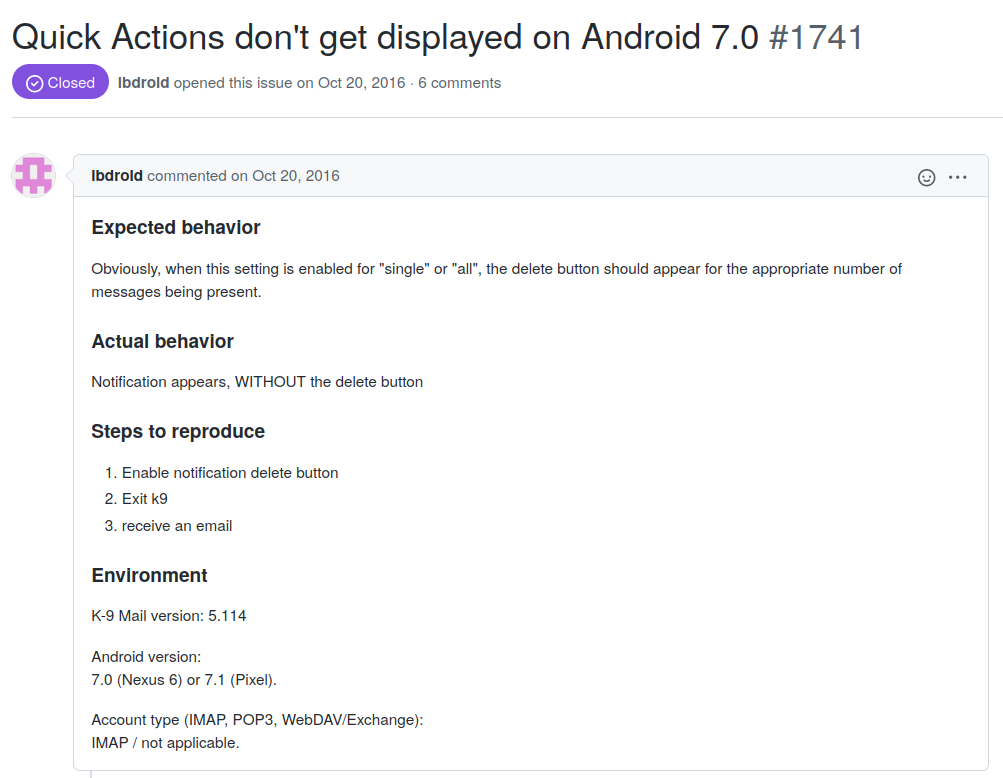
\includegraphics[width=\dimexpr\linewidth-4\fboxsep-2\fboxrule]{cp1/android-quick-actions}
     \caption{k-9 mail GitHub issue \#1741 indicating that quick actions don't get displayed on Android 7.0}
     \label{fig:android-notifications-task}
 \end{figure}
 
 
 \medskip
 A developer assigned to this issue might not be familiar with how Android notifications work and thus, they will need additional knowledge to understand and resolve the bug~\cite{ko2007, Li2013, sillito2006}. 
 More than often, this knowledge can be acquired from a developer's peers~\cite{singer2011}. 
 However, the fragmented and distributed nature of software development  
 may prevent the developer from accessing their peers~\cite{ko2007},
 instead they seek online web resources for information 
 that may assist them in completing the task-at-hand~\cite{Xia2017, rao2020}.
 
 
 
 
 
 \begin{figure}
     \centering
     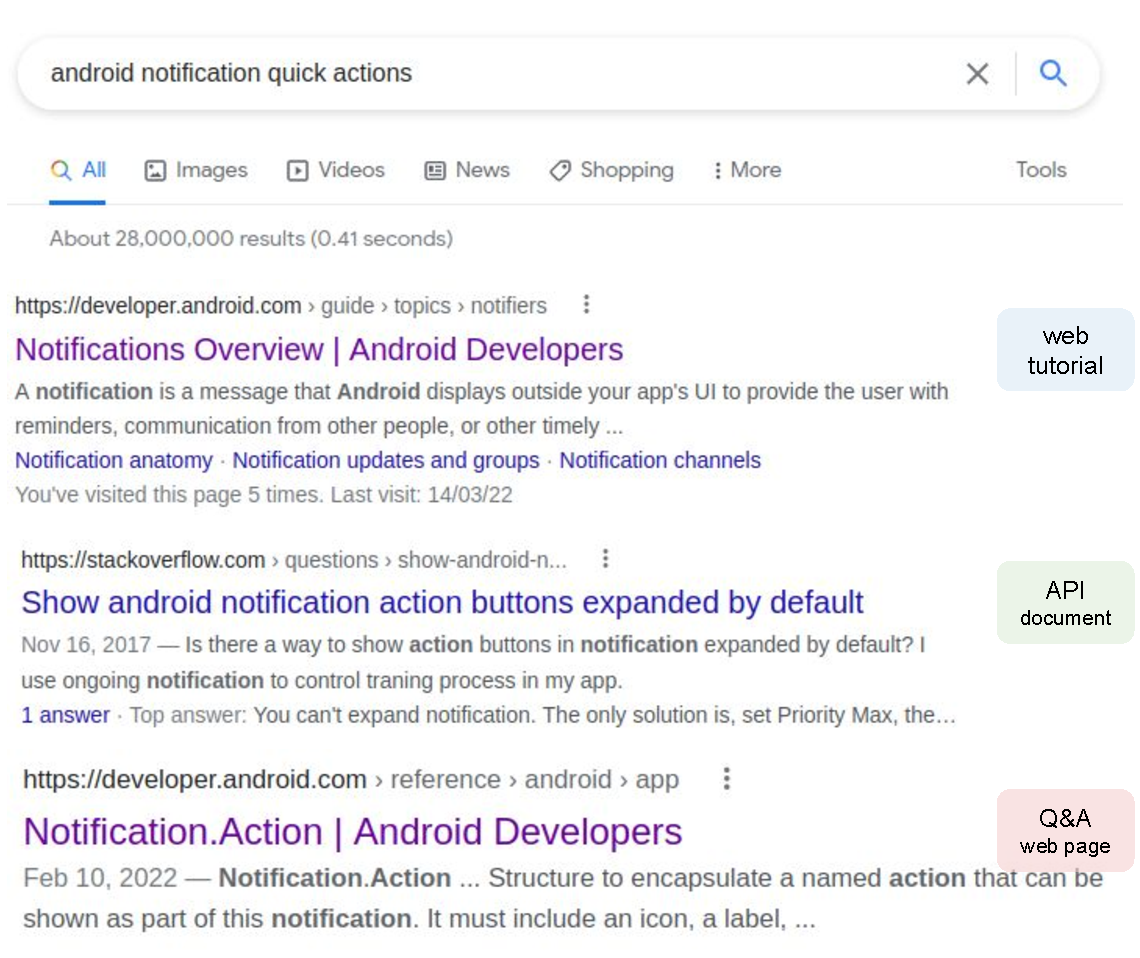
\includegraphics[width=.80\textwidth]{cp1/search-results.pdf}
     \caption{Search results showing artifacts of potential interest to the Android quick actions issue}
     \label{fig:android-search-results}
 \end{figure}
 
 
 
A common way to find software artifacts
pertinent to the developer's task
is through the usage of a web search engine~\cite{Brandt2009a, Li2013}.
Figure~\ref{fig:android-search-results}
shows the artifacts resulting from a developer's search 
about android notifications for the task in Figure~\ref{fig:android-notifications-task}.
We explain the information found in these artifacts
and challenges associated with locating 
task-relevant text within them as follows.



% https://tex.stackexchange.com/questions/339026/how-to-make-the-text-float-around-figures-in-landscape-mode
% https://tex.stackexchange.com/questions/468393/including-large-images-in-landscape-formatting


\afterpage{
\begin{landscape}
\begin{figure}
    \centering
    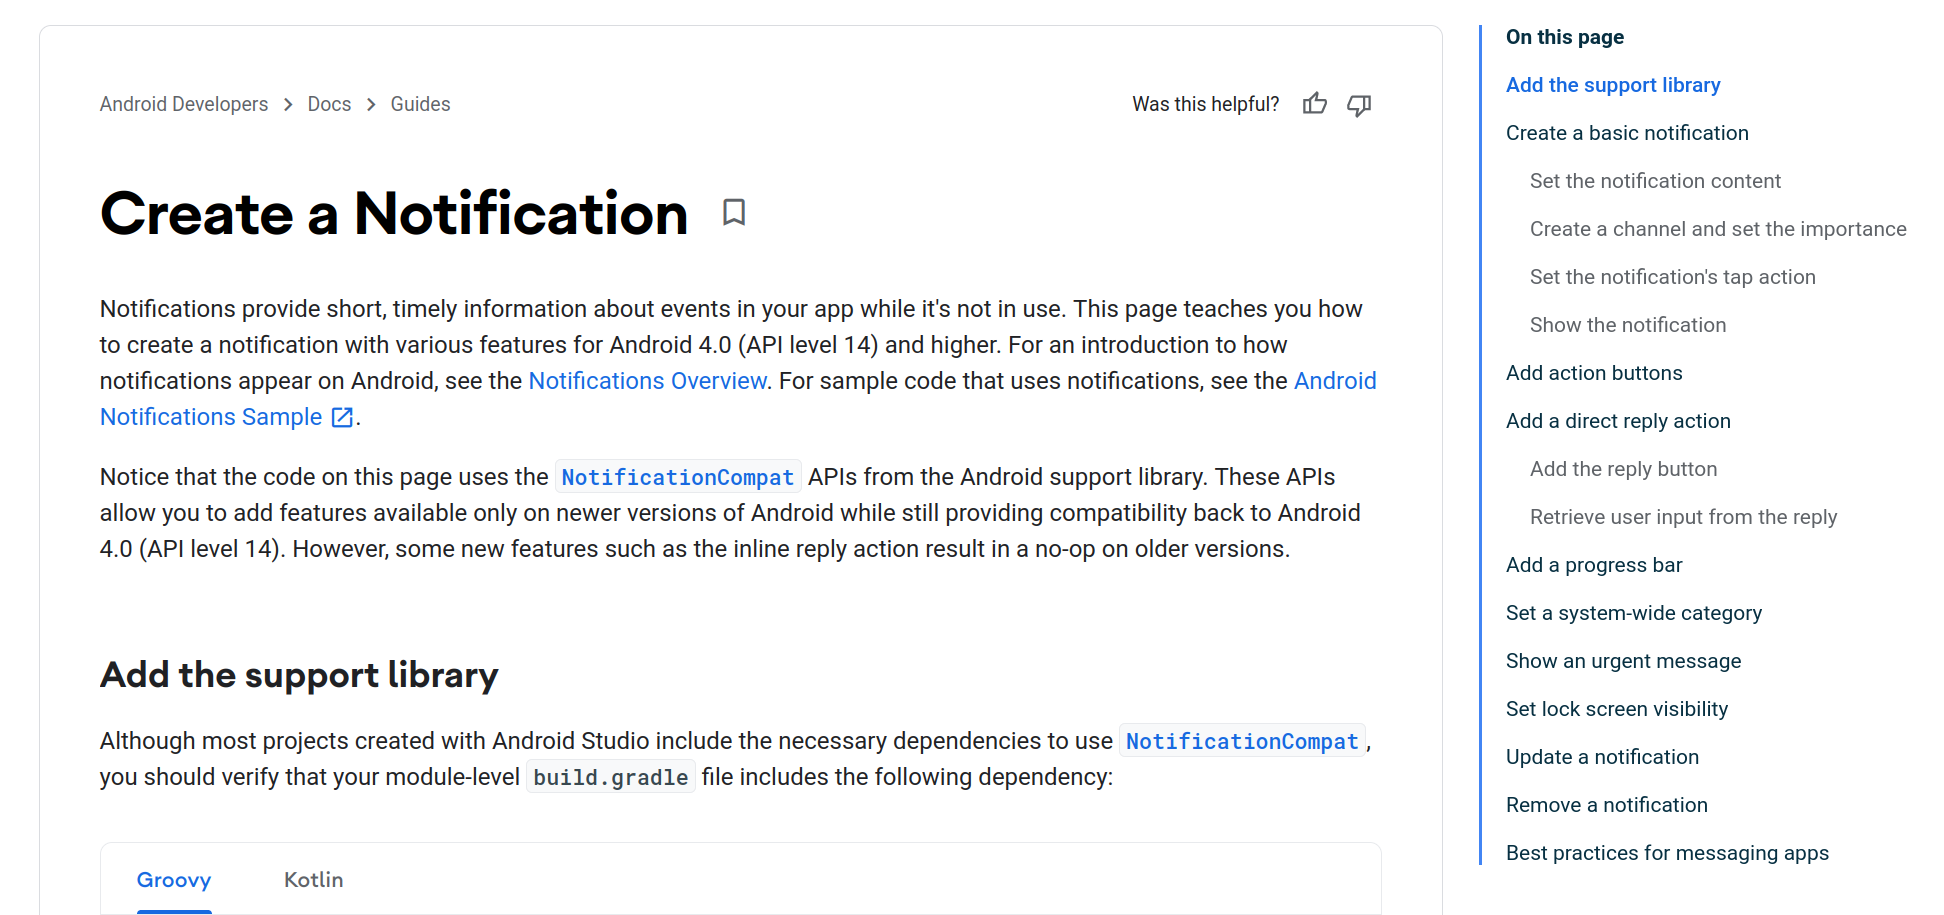
\includegraphics[width=\dimexpr\linewidth-4\fboxsep-2\fboxrule]{cp1/create-notification.png}
    \caption{Snapshot of the official Android notifications tutorial}
    \label{fig:android-create-notification}
\end{figure}
\end{landscape}
}

A web tutorial is a document intended primarily to teach users how to use 
a technology~\cite{arya2020}. 
% A technology provider might 
% provide a tutorial alongside standard API documentation or 
% the developers who use that technology can write independent tutorials on their own~\cite{Jiang2016b,Jiang2017}. 
As a learning resource, tutorials often contain a series of structure topics 
that progressively explain concepts about a certain technology~\cite{Jiang2016b, Jiang2017}. 
Figure~\ref{fig:android-create-notification} provides an example 
of an official tutorial for the Android notifications. 
This tutorial contains  approximately 200 sentences
and on the page's right-hand side, we find that this tutorial
has nine sections, each with sub-sections of their own. 
Reading all sections of this document could potentially 
take 10 minutes or more\footnote{Using a standard reading metric of 200 words per minute~\cite{Just1980}} of a developer's time 
and, to save time, a developer would likely try to find the sections of the document
most closely related to their task~\cite{Li2013}, but not without challenges.
For example, using a keyword search mechanism to find content within this web tutorial 
that mentions the `\textit{actions}' keyword, 
a developer would find eight different matches spread across four different sections
and even with a matching section, 
such as the `\textit{Notification actions}'
 (under focus in the figure), 
not all the text might be relevant to 
a developer.
That is, 
the section explains 
notifications for both Android version 7.0 and 12.0, what is expected from an artifact produced for a large audience
that may have different information needs, but given that the developer's task is related to the former version,
only the text highlighted (in orange)
might be of relevance to the task in Figure~\ref{fig:android-notifications-task}.






An \acf{API} defines how  two software libraries communicate~\cite{robillard2011field}.
For example, how the mail client software communicates 
with the native Android software. This communication happens via features and functionality exposed by the API~\cite{Robillard2015} 
and instructions about its usage are often found in the API's references documentation.
Figure~\ref{fig:android-notification-action} shows part of the reference documentation for one of the classes of the Android API, namely `\textit{Notification.Action}'. 
In the right-hand side of the figure, we find common 
information in this type of document, including a brief summary,
constants and fields available, the class' constructor, and 
each of the functions, or methods, that this particular class provides,  
for a total of 35 distinct elements.
To find the portions of the text relevant to
their task,
a developer unfamiliar with this document would 
face challenges similar to the ones  described in the web tutorial. Additionally, 
we note that complex APIs, 
such as Android, require combining several classes
and method calls~\cite{robillard2011field} to properly perform some instruction,
what would mean inspecting at least three other classes 
with equally complex documentation
to understand all the Android API elements used in the quick actions menu.





\begin{figure}
    \centering
    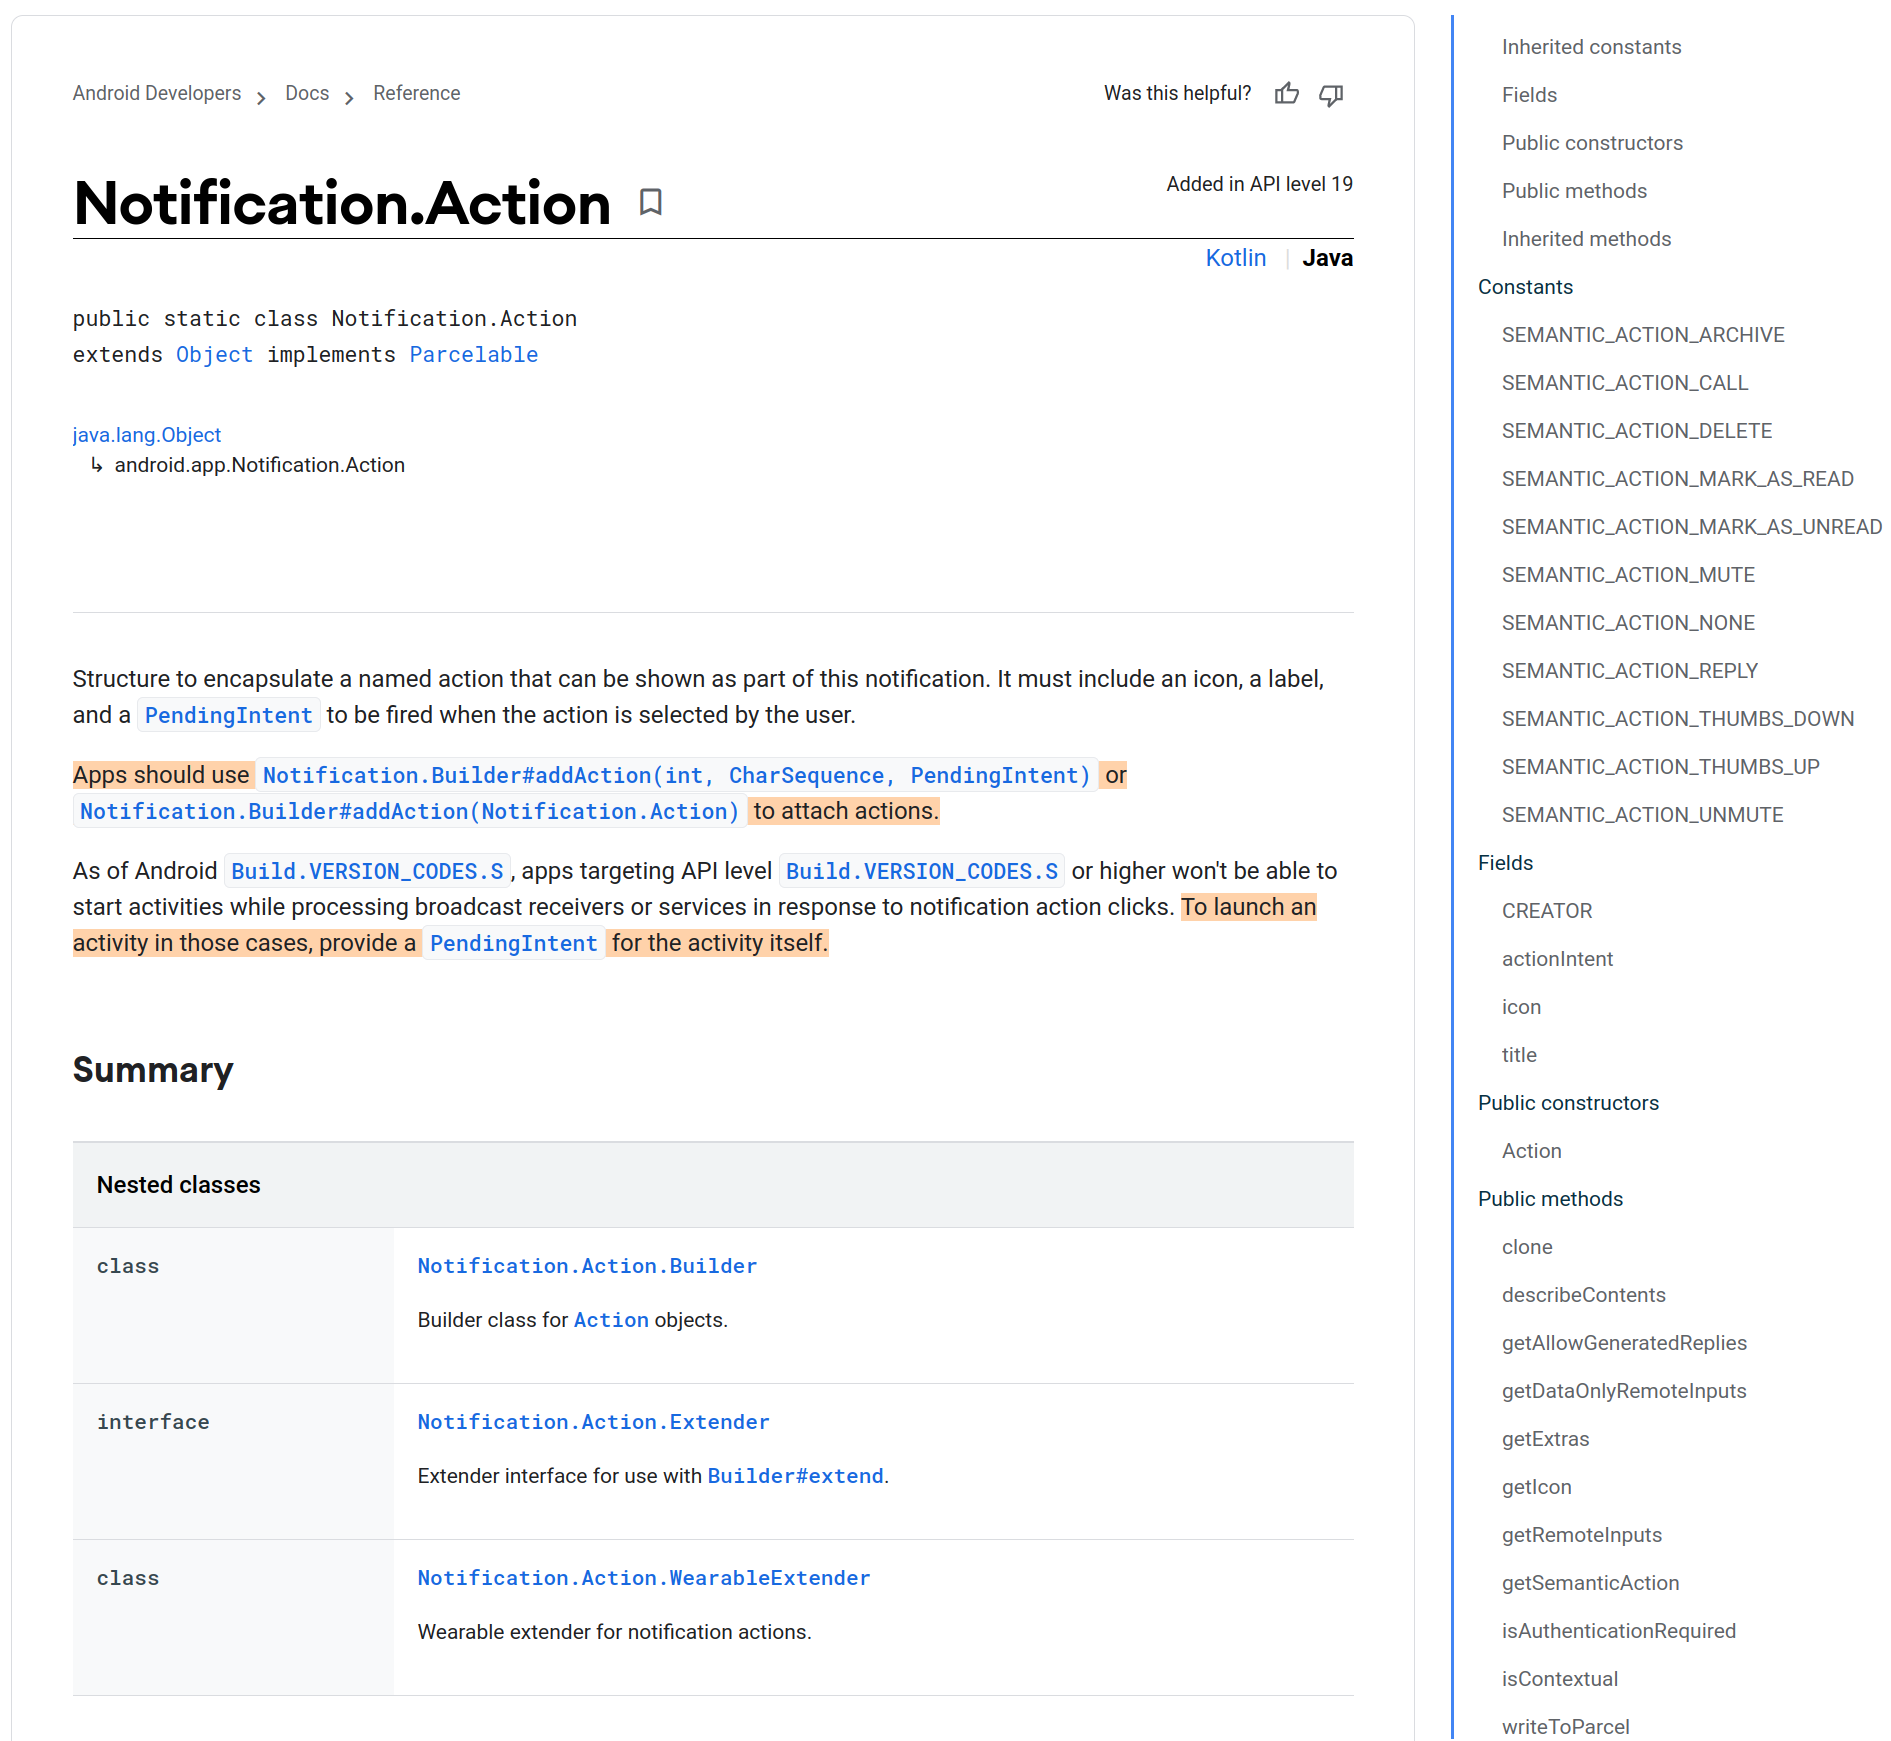
\includegraphics[width=\dimexpr\linewidth-4\fboxsep-2\fboxrule]{cp1/notification-action.png}
    \caption{Snapshot of the Android Notification.Action API reference documentation}
    \label{fig:android-notification-action}
\end{figure}




The third artifact resulting from the developer's search 
about android notifications (Figure~\ref{fig:android-search-results})
is a post in a \acf{qa} web portal, namely Stack Overflow\footnote{\url{https://stackoverflow.com/}}.
Figure~\ref{fig:qa-notification-icon} shows an example of the information found in this type of artifact.
A question usually contains both text and code sniptes
and it includes a set of tags  about the
problem's programming language and technology~\cite{Treude2011a}. 
Each answer contains similar content; 
the counter that appears on left of a question and of each answer
represents whether other users found them helpful (or not).
The user who asked the question can also accept an answer (green check mark)
if it correctly solved their problem
and we find a list of similar or related questions 
at the right portion of the page. 
For this type of artifact, a developer would ideally read the problem and 
then a accepted answer to quickly find information that might be helpful 
to their task, but a series of factors make finding useful information challenging. 
For example, only half of the Android questions on Stack Overflow
have an accepted answer~\cite{parnin2012} 
and millions of questions have more than one answer~\cite{nadi2020}.
Technologies also evolve and answers become obsolote~\cite{Allamanis2013}.
Hence, despite the fact that structured data (i.e., votes and accepted answers) might 
assist a developer
in their search, finding task-relevant text in this type of artifact is also not 
trivial.




\begin{figure}
    \centering
    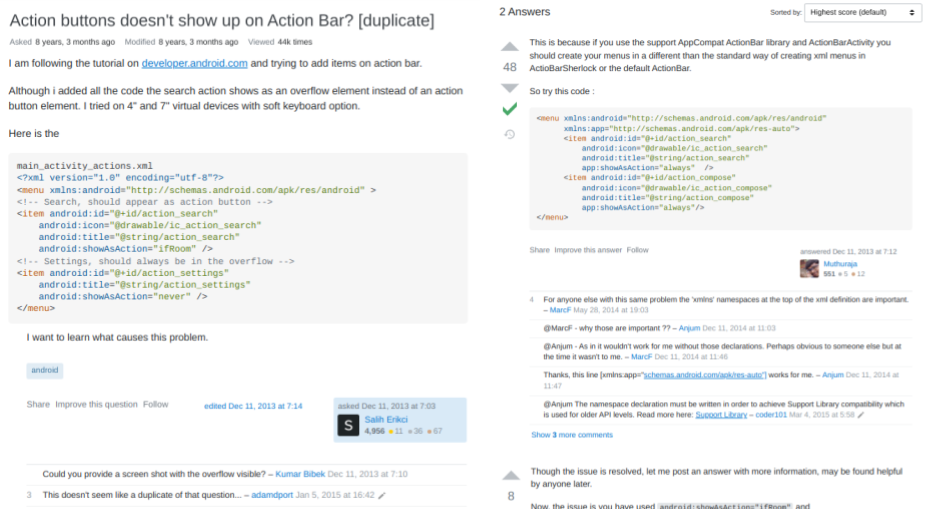
\includegraphics[width=\dimexpr\linewidth-4\fboxsep-2\fboxrule]{cp1/stackoverflow-notifications.png}
    \caption{Snapshot of a Stack Overflow question about Android notifications}
    \label{fig:qa-notification-icon}
\end{figure}



At this point, it is clear that if no tool support is provided, much of the process of navigating through a natural language artifact and  locating text 
relevant to a task falls on the developer's shoulders~\cite{gonccalves2011, Ko2006a, Bystrom1995} and, given how quickly developers progress to use new kinds of technology to
record pertinent information, the challenges we outlined are not exclusive 
to the three types of artifact in Figure~\ref{fig:android-search-results}, rather 
they are common to many kinds of natural language software artifacts.




 \clearpage
 
 
 
%  As tasks become more complex~\cite{Pirolli2007, Bystrom1995}, a developer also has to combine multiple textual fragments---from the same artifact or from different ones---to understand what is needed for the task-at-hand~\cite{Piorkowski2016}. 
%  For example, the information within the web tutorial 
%  might have only partially assisted the developer in understanding how 
%  Android notifications work and thus, they would consult other artifacts from their search for more information, namely the API document and \acs{qa} web page. 
%  Figure~\ref{fig:anatomy-of-relevant-text} gives further insight into 
%  how task-relevant text 
%  is scattered across these other artifacts. 
%  From the figure, we find that some of the text potentially relevant to this task (in orange) is attached to elements that a reader would not intuitively access~\cite{Robillard2015}, i.e., 
%  a sentence at the end of a paragraph or a comment under the original question,
%  and if no tool support is provided, much of the process of finding this relevant text falls on the developer's shoulders~\cite{gonccalves2011, Ko2006a, Bystrom1995}.
 
 
 
%  Researchers have long recognized the value of 
%   assisting developers in locating information in the natural language artifacts sought as part of a software task,
%  proposing many tools and approaches 
%  that combine \acf{IR}, \acf{NLP} and \acf{ML} techniques to identify potentially useful text in certain kinds of artifacts. 
%  For example, Nadi and Treude consider 
%  that relevant information in \acs{qa} 
%  web pages are often found in text with
%  conditional clauses (i.e., sentences with the word `\textit{if}')~\cite{nadi2020}
%  while Robillard and Chhetri assume that relevant 
%  text in API documents mention a code element such as a class name or method signature~\cite{Robillard2015}; they use such assumptions 
%  in techniques that identify this text automatically.
%  As other examples, both Xu et al.~\cite{Xu2017} 
%  and Silva et al.~\cite{silva2019} use 
%  meta-data available on each of the answers in a Stack Overflow post 
%  as a proxy for relevant information.
%  That is, they use the number of votes an answer has or the checkmark indicating if an answer is the correct one, both shown in Figure~\ref{fig:anatomy-of-relevant-text}, 
%  to automatically identify text that might be relevant to a given task in these answers. 
 
 

% % https://tex.stackexchange.com/questions/468393/including-large-images-in-landscape-formatting
% \begin{landscape}
% \begin{figure}
%     \centering
%     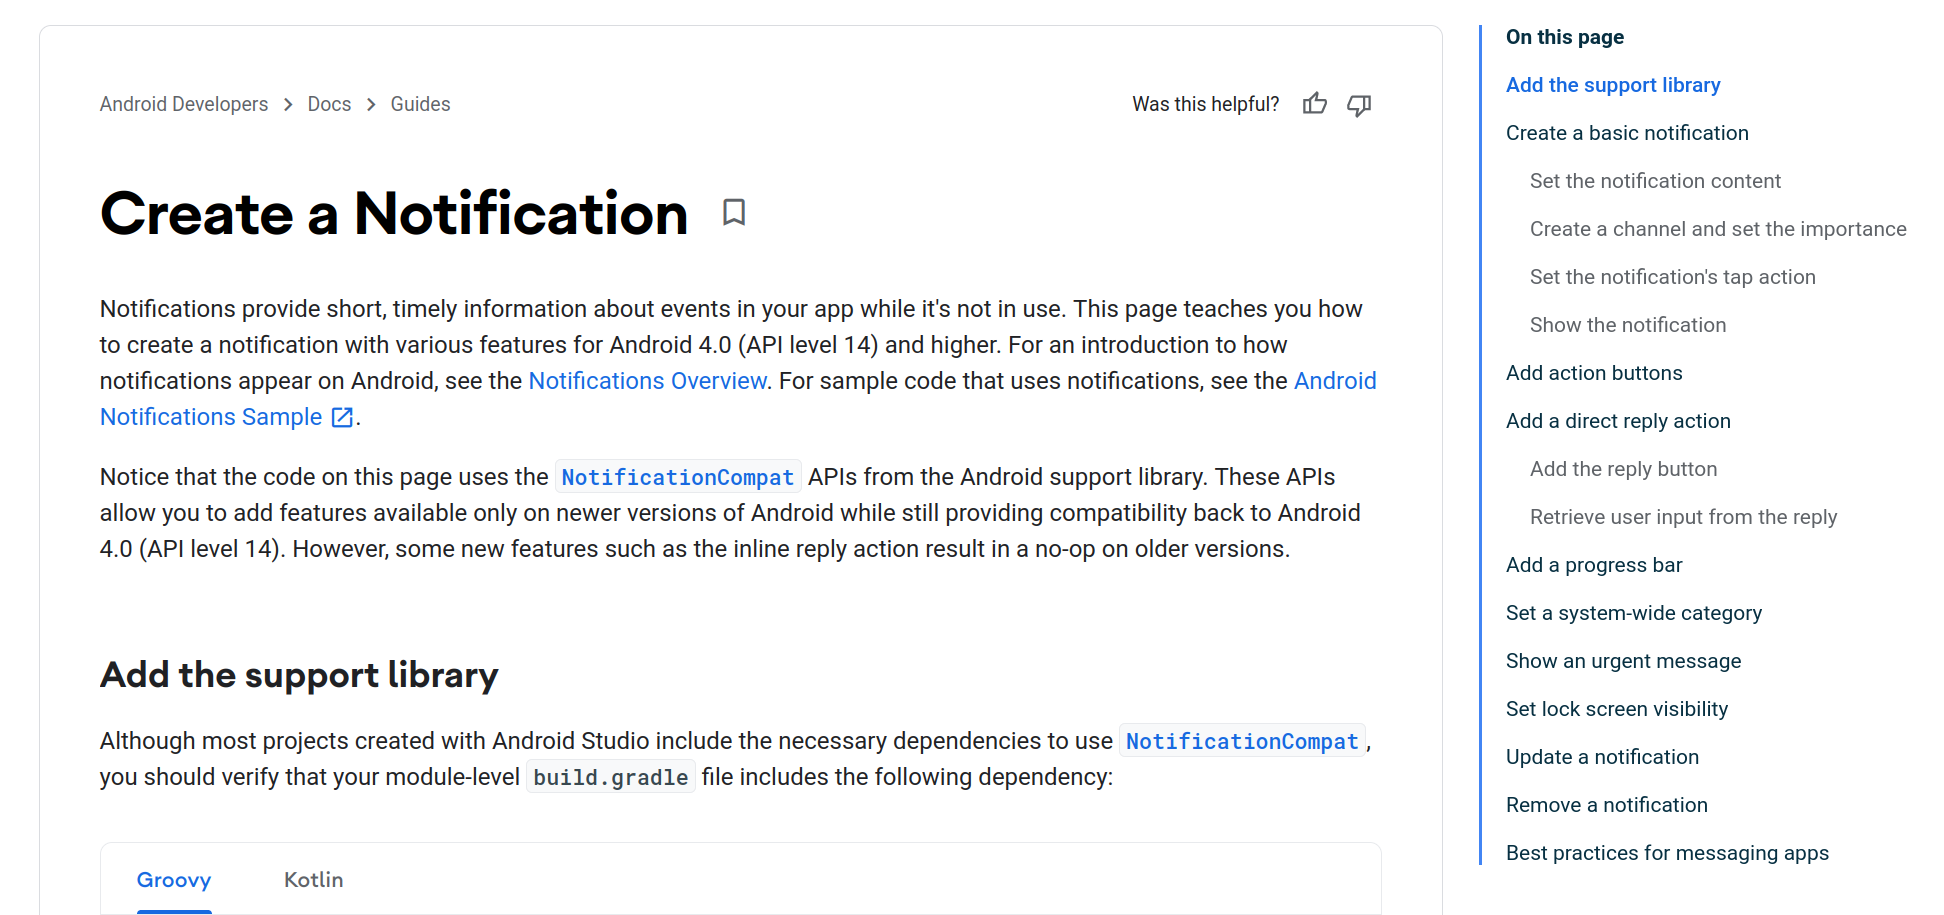
\includegraphics[width=\dimexpr\linewidth-4\fboxsep-2\fboxrule]{cp1/create-notification.png}
%     \caption{Snapshot of the official Android notifications API overview}
%     \label{fig:android-create-notification}
% \end{figure}
% \end{landscape}
    

 
 
 

% \begin{landscape}
% \begin{figure}
%     \centering
%     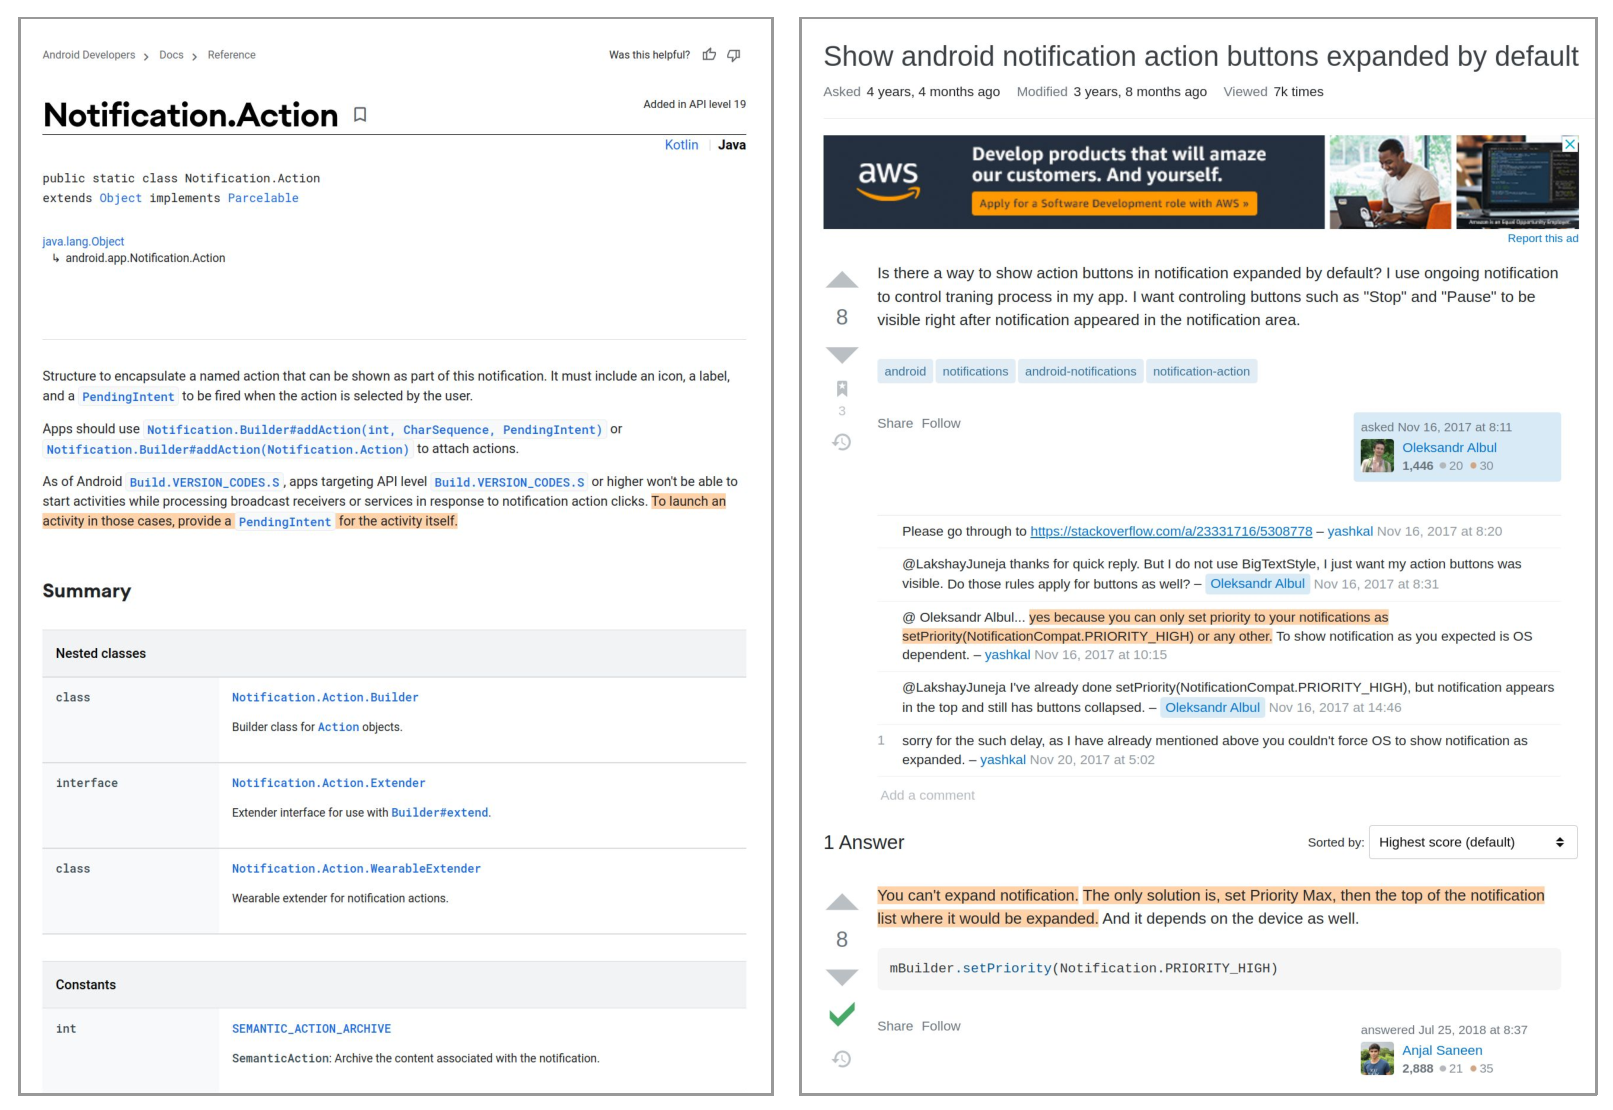
\includegraphics[width=\dimexpr\linewidth-4\fboxsep-2\fboxrule]{cp1/notifications-relevance-2.pdf}
%     \caption{Relevant text for the Android notifications task found across different kinds of artifacts, i.e., an API document (on the left) and a question-and-answer web page (on the right)}
%     \label{fig:anatomy-of-relevant-text}
% \end{figure}
% \end{landscape}

 
 
 
%  Although effective in specific contexts,
%  it is reasonable to assume that these techniques might not apply 
%  to the different kinds of artifacts. This is either because these techniques have  assumptions on the nature of relevant text that do
%  not extend to the text found in other types of artifacts, or 
%  because these techniques rely on 
%  meta-data, which is only available in specific kids of artifacts
%  and given how quickly developers progress to using new kinds of technology to
%  record pertinent information (e.g., slack~\cite{Storey2017, Lin2016}),
%  it may be difficult to scale such artifact-centric approaches to cover the range of
%  artifacts that 
%  a developer may encounter
%  daily in their work~\cite{Li2013}.
 
 
 
 
 




% \clearpage


% a snapshot 
% of the Android notifications documentation, where among  
% the many topics presented on the page (right-hand side), only the `\textit{notification actions}' portion (under focus) might be rof relevance.
% This illustrates the burden of sifting through large amounts of
% irrelevant text (e.g., because of legacy information, boilerplate text, or because it is intended for another audience) to filter just those parts that are relevant to a developer~\cite{Robillard2015}. 











% about adding
% action to a notification is found across multiple artifacts.
% If no tool support is provided, much of the process of navigating through artifacts of interest and locating text 
% relevant to a task fall on the developer's shoulders~\cite{gonccalves2011, Ko2006a, Bystrom1995}.






% Researchers have long recognized the value of assisting developers in 
% identifying information of relevance within the natural language
% text of a software artifact






% but such a technique would fail to locate the relevant text 
% shown in Figure~\ref{fig:anatomy-of-relevant-text}.


% consider pre-defined kinds of tasks or types of artifacts.
% For example, {\small DeMIBuD}~\cite{Chaparro2017} is a technique that applies to bug reports and 
% assists in bug triaging. Although valuable, the text   detailing a bug's observed or expected
% behaviour and automatically identified by this tool
%  is of little help to a developer who accessed that bug 
% with the hope that the bug's solution also applies to their current task~\cite{Viviani2019}.





% 
\vspace{3mm}
\begin{figure}
\centering    
\parbox{\textwidth}{% 
\centering
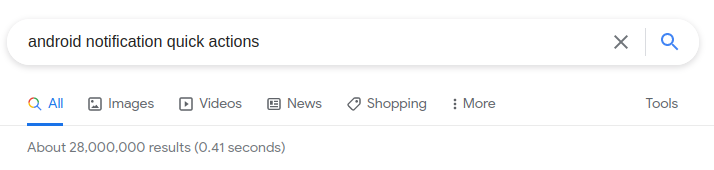
\includegraphics[width=.80\textwidth]{cp1/task-google-search}
}
\parbox{\textwidth}{%
\centering
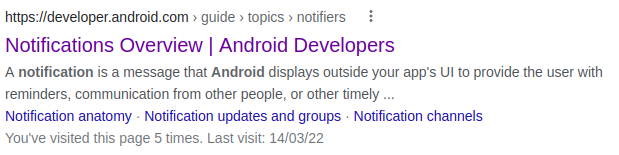
\includegraphics[width=.70\textwidth]{cp1/api-documentation-search-result}
}
\parbox{\textwidth}{%
\centering
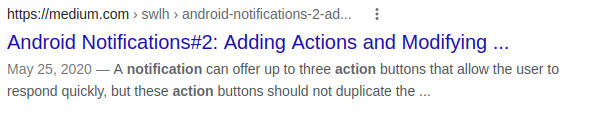
\includegraphics[width=.70\textwidth]{cp1/misc-documentation-search-result}
}
\parbox{\textwidth}{%
\centering
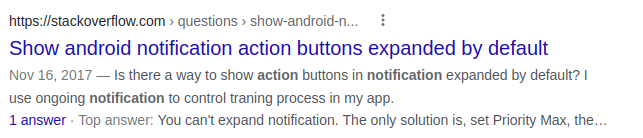
\includegraphics[width=.70\textwidth]{cp1/so-documentation-search-result}
}
\parbox{\textwidth}{%
\centering
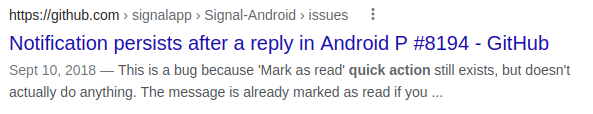
\includegraphics[width=.70\textwidth]{cp1/git-documentation-search-result}
}
\caption{Search results showing artifacts of potential interest to the Android quick notifications issue}
\label{fig:android-search-results}
\end{figure}







% While it is impractical to anticipate all the information needs a developer might have~\cite{sillito2006, josyula2018, ko2007}, there is an increasing interest in using the information 
% available in a software task for the purposes of automatically identifying text 
% which might assist in completing that task~\cite{Bavota2016}. 
% In such context, most of the approaches proposed by software engineering researchers 
%  only apply to certain kinds of artifacts, such as Stack Overflow posts~\cite{Xu2017, silva2019}, 
%  and use structural data available in these artifacts (e.g., extracting text only from top ranked answers)  to assist in the identification of relevant text
 
% These assumptions limit using such techniques across the
% many different kinds of artifacts a developer may encounter
% daily in their work~\cite{Li2013}, 
% illustrating thus some of the challenges in locating task-relevant textual
% information and motivating the need for more generalizable techniques.





% \begin{landscape}
% \begin{figure}
%   \centering
%   \begin{minipage}{.5\textwidth}
%       \centering
%       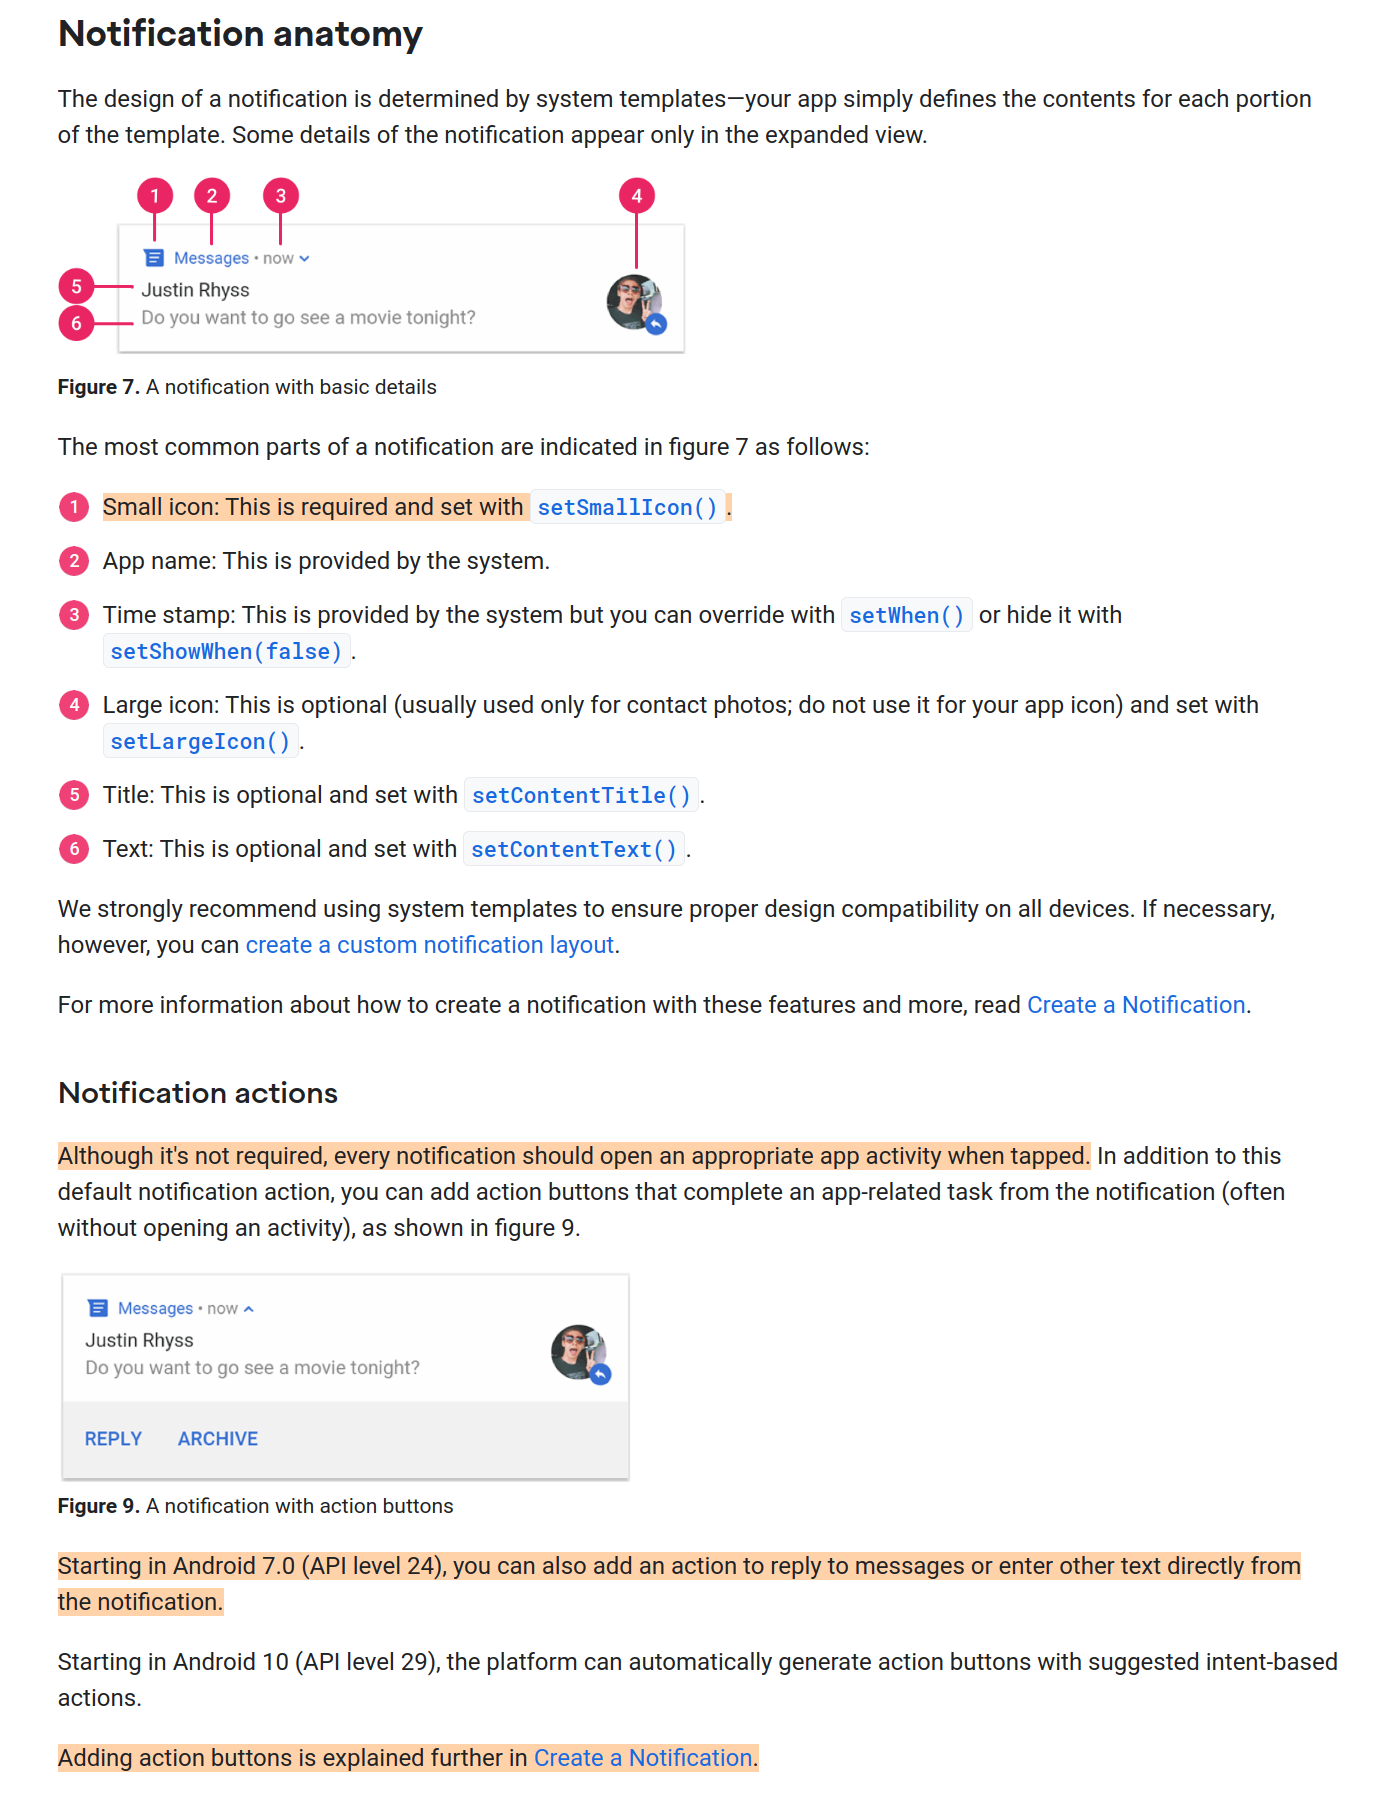
\includegraphics[width=0.5\linewidth, height=0.2\textheight]{cp1/notification-anatomy}
%     %   \caption{The Skip-gram model architecture~\cite{Mikolov2013}}
%     %   \label{fig:skip-gram}
%   \end{minipage}%
%   \begin{minipage}{0.5\textwidth}
%       \centering
%       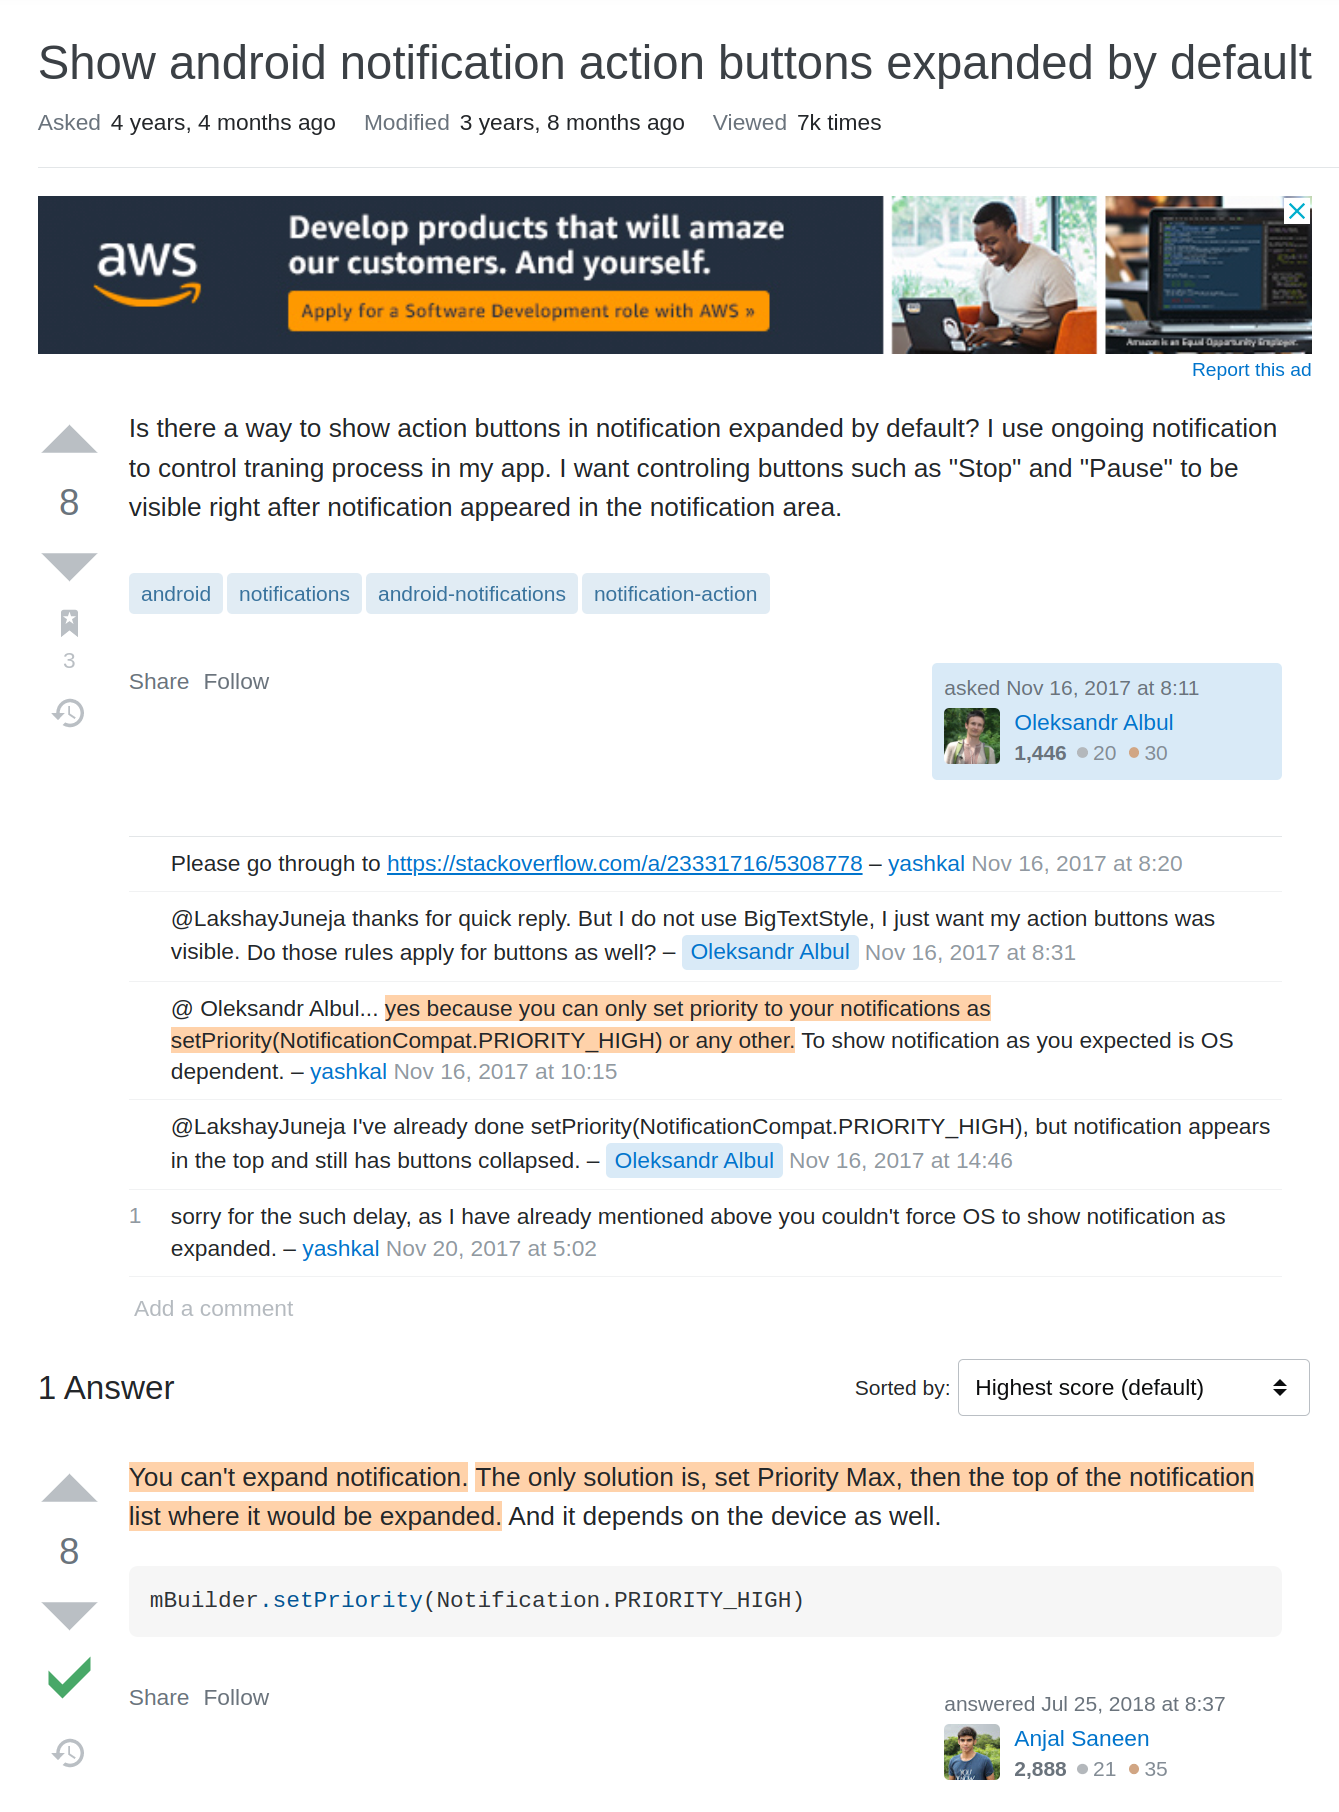
\includegraphics[width=\linewidth, height=0.2\textheight]{cp1/expand-notifications}
%     %   \caption{Positive and negative training examples~\cite{Ye2016}}
%     %   \label{fig:skip-gram-example}
%   \end{minipage}
% \end{figure}
% \end{landscape}





% Some \acs{NLP} techniques rely on regular expressions describing a sequence of tokens
% representing words or linguistic elements 
% often found in relevant text~\cite{Bavota2016, Chaparro2017}.
% Other \acs{ML}-based techniques use extractive text summarization 
% to produce a summary of an artifact's content~\cite{Lotufo2012, Ponzanelli2015}
% and a developer might use this summary to find key information
% that may help them complete their task~\cite{Bavota2016}.